\hypertarget{Microfacet Models}{
}

\noindent In the previous section, the reflection models were based on emperical observations. Research in optics found that these models deviate from reality in a number of aspects. In this section, a more physically correct class of reflection models will be outlined. They are called \textit{first principlces} models because they apply basic laws of physics on a microscopic scale. The interaction of light on this microscopic scale in turn determines how the light gets reflected from the surface. The light interaction could be described by either wave or geometric optics, but only geometric optics based models are discussed in this research.

The models described here start by modeling the surface geometry at microscopic scale. Rather than providing an exact description of this structure, the assumption is made that the surface varies randomly in height and orientation of facets. With this assumption, its possible to use statistical models to model surface structures.

\section{Surface Roughness Model}
There are two possible methods to represent the random surface. Both methods use small differently oriented areas in their representation, also called microfacets. The first method is to model the surface using a random process such as described by Beckmann and Spizzichino \cite{BeckmannSpizzichino}. They suggest to build the surface by using coin-flipping to decide to increase, decrease one or two units or stay on the same level. Although the resulting surface will have a desirable randomness, it is very complex to derive reflectance models using this method. 

The second method uses primitive shapes to describe the surface. Torrance and Sparrow suggested to represent the surface as a composition of symmetric V-cavaties, where each microfacet has a height much bigger than their width and the upper edges are all laying in the same plane. With the assumption $\lambda^2 \ll da \ll dA$, where wavelenght of light $\lambda$ is much smaller than the facet area $da$, and the facet area $da$ is much smaller than the area $dA$ (which is a pixel on the surface), geometric optics can be used to derive the reflectance models.

\section{Geometric Optics}
The idea of describing the surface as a collection of microfacets is originally developed in the field of optics and radiation tranfer. Microfacets with respect to computer graphics has first been addressed by Blinn \cite{Blinn}. He proposed that a model for computer simulation could be composed from the following factors:

\begin{itemize}
	\item{ The number of microfacets are facing the orientation of the viewing direction, and what is the projected area of the facets into the viewing direction. This is computed by the slope distribution function. }
	\item{ How much incoming light on a microfacet gets blocked by other microfacets, causing shadows to appear on the blocked microfacet when observing the microfacet from certain angles (see figure X).} 
	\item{ How much reflected light into the viewing direction gets blocked by other microfacets, causing the amount of radiance reaching the viewer to be smaller than the amount of radiance that gets reflected from the microfacet. This phenomenom is called masking, and is also shown in figure X. }
	\item{ How much can an unobstructed microfacet reflect? This is mainly dependent on a given reflectance function for the microfacet. This is general is either Lambertian or pure specular. See figure X for an example using pure specular reflectance}
\end{itemize}

The shadowing and masking of the microfacets need additional geometric analysis next to the slope distribution. The most common way to deal with this analysis is to assume that the microfacets form V-shaped cavaties as shown in the example images. This approach has been challenged since the assumption is inconsistent with the assumption of a random looking surface, but it makes geometric analysis much easier.

Another case of geometric analysis which can be included, is the phenomenom of interreflection. This happens when radiance is being exchanged between two diffuse surfaces, and causes the effect of color bleeding. The analysis is included in the reflection model proposed by Oren and Nayar, and is described in section \ref{sec:OrenNayar}.

\begin{figure}[H]
	\begin{center}
		\subfigure[Unblocked]{
\epsfig{file=images/microfacets_full_reflection.eps, width=0.4\linewidth}}\label{fig:GAFa}
		\subfigure[Shadowing]{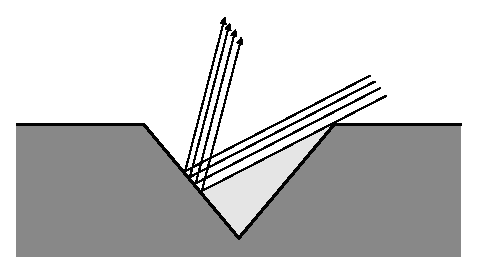
\epsfig{file=images/microfacets_shadowing.eps, width=0.4\linewidth}}\label{fig:GAFb}
		\subfigure[Masking]{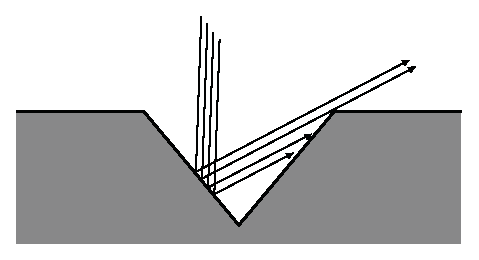
\epsfig{file=images/microfacets_masking.eps, width=0.4\linewidth}}\label{fig:GAFc}
		\subfigure[Interreflection]{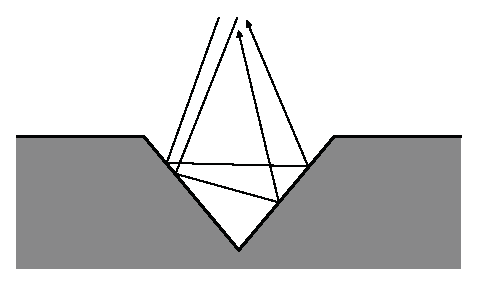
\epsfig{file=images/microfacets_interreflection.eps, width=0.4\linewidth}}\label{fig:GAFd}
	\end{center}
	\caption{Four cases of light interaction on microfacets.}
	\label{fig:GAF}
\end{figure}


\section{Torrance-Sparrow Reflectance}\label{sec:CookTorrance}
	The results of experiments conducted by Sparrow and Torrance \todo{reference} showed that Phong reflectance does closely simulates the behavior of speculars on shiny/glossy surfaces. However, some differences were reported, with the main difference being that the specular bump varies with the direction of the light source. Also, the specular reflection is not always reflected in the halfway vector H. 

Torrance and Sparrow derived models to explain these differences, and Blinn translated these models to be useful in computer graphics. The specular component can be described as a function of four factors: 
	
	\begin{eqnarray*}
%		f = \frac{F(\theta_h)D(\theta_h)G(\theta_i,\theta_r)}{\pi \cos(\theta_i) \cos(\theta_r)}
		s = \frac{F(\theta_h)D(\theta_h)G(\theta_i,\theta_r)}{\vec{\mathbf{n}} \cdot \vec{\mathbf{e}}}
	\end{eqnarray*}

where $D$ is the distribution function of the directions of the microfacets. Each microfacet is assumed to be perfectly specular. $G$ contributes the amount of light that gets masked and/or shaded by other microfacets, and $F$ is the Fresnel reflection law.

Taking into account that the observer sees more of the microfacet surface area when the surface is tilted, this tilt angle is included in the division in the above equation as $\vec{\mathbf{n}} \cdot \vec{\mathbf{e}}$, since this observed area is inversely propportional to the cosine of the tilt angle.

The distribution function used by Torrance and Sparrow was a simple Gaussian function, $D = e^{-(\alpha c)^2}$, where $c$ is the standard deviation and $D$ is the amount of microfacets oriented at an angle $\alpha$, the angle between the facing direction of the microfacets and the surface normal. Since we are only interested in the microfacets pointing into the direction of $\vec{\mathbf{h}}$, the angle $\alpha = \theta_h$. Blinn used a different function however, developed by Trowbridge and Reitz, and suggests modeling the microfacet distribution as ellipsoids:

	\begin{eqnarray*}
		D_{Blinn}(\theta_h) = \left({ \frac{m^2}{\cos^2(\theta_h)(m^2-1)+1} } \right)^2
	\end{eqnarray*}

In the above equation, the parameter $m$ controls the eccentricity of the ellipsoid. When set to 0, the distribution defines a shiny surface, and when set to 1, it defines a rough surface.

The factor $G$ in the specular reflection equation accounts for the effect of masking and shadowing of microfacets. This factor is also called the \textit{geometrical attenuation factor}, and gives a value between 0 and 1 to represent the amount of light remaining after shadowing/masking. The method described by Blinn to calculate this factor assumes symmetrical identical V-shaped cavities as stated earlier. 

The three cases are included in the geometrical attenuation factor. For arbitrary light source directions and viewing directions, the three cases that can happen are shown in figure \ref{fig:GAF}.

The first case is that of figure \ref{fig:GAFa}a, where no light is obstructed by other microfacets and therefore there is no attenuation. In this case, the attenuation is defined as:

	\begin{eqnarray*}
		G_a = 1
	\end{eqnarray*}

In the case of figure \ref{fig:GAFb}b, some of the incident light gets intercepted when traveling to the observer. For this case, the attenuation is defined as follows:

	\begin{eqnarray*}
		G_b = \frac{2\cos(\theta_h)\cos(\theta_r)}{\cos(\theta_{rh})}
	\end{eqnarray*}

Because the same concept applies for figure \ref{fig:GAFc}c, but the light and view source are interchanged, the final attenuation can be defined as:

	\begin{eqnarray*}
		G_c = \frac{2\cos(\theta_h)\cos(\theta_i)}{\cos(\theta_{rh})}
	\end{eqnarray*}

For the exact derivation of these individual terms, the work of Blinn \cite{Blinn} can be consulted. For the implementation of $GAF$, the minimum of all three cases is used as the effective value for $G$:

	\begin{eqnarray*}
		G = min \left[ {G_a, min \left[ {G_b, G_c} \right] } \right]
	\end{eqnarray*}

The final term in the specular reflection equation is the Fresnel term. This term gives the fraction of light that is reflected from a microfacet instead of being absorbed. An object's surface is considered an interface between two different substances; the object's substance and the substance the object is surrounded with (eg. water or in this case air). The Fresnel equations, developed by Augustin-Jean Fresnel in the 19th century, describe an optical property such that reflected light is not only dependent on the incoming light angle $\theta_i$, but also on the \textit{refraction index} of both substances. The exact Fresnel equations are quite complex and need correct refraction indices which are not available for the PhoTex database. 

A simplified version of the Fresnel equations is given by Schlick \cite{Schlick}, which is proven to be fairly accurate for a lot of substances and is given by the equation:

	\begin{eqnarray*}
		F(\theta_i) = R_f(0^o) + (1 - R_f(0^o))(1 - \cos(\theta_i))^5
	\end{eqnarray*}

in this equation, $R_f(0^o)$ represents the specular color of a substance when the incident light strikes the surface under an anlge of $\theta_i = 0$. This value for $R_f(0^o)$ is typically low for dielectrics such as plastic, stone, wood, concrete, leather, etc. and is measured around 0.05 or lower \cite{RTR}. 


\section{Oren-Nayar Reflectance}\label{sec:OrenNayar}
A big deficiency in approximating the body reflectance under the Lambertian assumption is that its view independent. This results in inaccurate approximations for several real-world objects, as experiments have demonstrated on several rough diffuse surfaces such as plaster, sand and cloth \cite{OrenNayar}. The main issue with Lambertian reflection for diffuse objects is that it creates high contrasts around the occluding boundaries of an object (such as a clay vase).

To overcome this deficiency, M. Oren and S.K. Nayar propose a more general reflection model for diffuse surfaces \cite{OrenNayar}, which borrows ideas from modelling the surface as a collection of microfacets as proposed for the Cook-Torrance or Torrance-Sparrow models. Microfacets are assumed to be perfectly Lambertian in reflection. This doesn't imply that surfaces are reflecting perfectly Lambertian however, since combination of all factors included produces accurate diffuse reflection also for non-Lambertian diffuse surfaces.

In their original paper, Oren and Nayar discussed various slope distributions for the representation of surface of microfacets. Using an uni-directional single-slope distribution (representing an anisotropic surface), they derive a geometric attenuation factor similar to that derived by Blinn. Also, a term for interreflections is introduced, where light rays bounce between adjacent facets. Since the energy of a light ray diminishes quickly on Lambertian surfaces, the interreflection uses up to two bounces. 



	\begin{eqnarray*}
		L_r^1 = \frac{\rho}{\pi}L_i\cos(\theta_i)\left[C_1+\cos(\phi_r-\phi_i)C_2\tan(\beta)+
			(1-|\cos(\phi_r-\phi_i)|)C_3\tan\left(\frac{\alpha+\beta}{2}\right)\right]
	\end{eqnarray*}

with the coefficients defined as:

	\begin{eqnarray*}
		C_1 = 1 - 0.5\frac{\sigma^2}{\sigma^2+0.33}
	\end{eqnarray*}

	\begin{eqnarray*}
		C_2 =
			\begin{cases}
				0.45\frac{\sigma^2}{\sigma^2+0.09} 		& \quad \text{if $\cos(\phi_r - \phi_i) \geq 0$}\\
				0.45\frac{\sigma^2}{\sigma^2+0.09} \left( \sin(\alpha) - \left( \frac{2\beta}{\pi}\right)\right) 	& \quad \text{otherwise}\\
			\end{cases}
	\end{eqnarray*}

	\begin{eqnarray*}
		C_3 = 0.125 \left( \frac{\sigma^2}{\sigma^2+0.09} \right)\left( \frac{4\alpha\beta}{\pi^2} \right)
	\end{eqnarray*}

The same approach of finding a good approximation accounts for defining the interreflection term:

	\begin{eqnarray*}
		L_r^2 = 0.17\frac{\rho^2}{\pi}L_i\cos(\theta_i)\frac{\sigma^2}{\sigma^2+0.13}\left[1-\cos(\phi_r-\phi_i)\left( \frac{2\beta}{\pi} \right)^2 \right]
	\end{eqnarray*}

